\documentclass[11pt,spanish,a4paper]{article}
% Versión 2.o cuat 2015 Víctor Bettachini < bettachini@df.uba.ar >

\usepackage{babel}
\addto\shorthandsspanish{\spanishdeactivate{~<>}}
\usepackage[utf8]{inputenc}
\usepackage{float}

\usepackage{units}
\usepackage[separate-uncertainty=true, multi-part-units=single, locale=FR]{siunitx}

\usepackage{amsmath}
\usepackage{amstext}
\usepackage{amssymb}

\newcommand{\pvec}[1]{\vec{#1}\mkern2mu\vphantom{#1}}

% \usepackage{tikz}
% \input{DimLinesTikz}
% \usetikzlibrary{decorations.pathmorphing, patterns}

\usepackage{graphicx}
\graphicspath{{./graphs/}}
\usepackage{wrapfig}


\usepackage[margin=1.3cm,nohead]{geometry}
% \voffset-3.5cm
% \hoffset-3cm
% \setlength{\textwidth}{17.5cm}
% \setlength{\textheight}{27cm}

\usepackage{lastpage}
\usepackage{fancyhdr}
\pagestyle{fancyplain}
\fancyhead{}
\fancyfoot{{\tiny \textcopyright Departamento de Física, FCEyN, UBA}}
\fancyfoot[C]{ {\tiny Actualizado al \today} }
\fancyfoot[RO, LE]{Pág. \thepage/\pageref{LastPage}}
\renewcommand{\headrulewidth}{0pt}
\renewcommand{\footrulewidth}{0pt}

% lista multicolumna
\usepackage{multicol}

% textsubscript
\usepackage{changes}

% \def \materia {Física II para químicos}
\def \periodo {cuatrimestre de verano - 2017}
\def \website {http://materias.df.uba.ar/f2qa2017v}


\begin{document}
\noindent
\textbf{Física II (Químicos)}\hfill \textcopyright {\tt DF, FCEyN, UBA}
% \textbf{\materia}\hfill \periodo
\begin{center}
  \textsc{\large Interferencia - División de frente de onda - División de amplitud}
  % \textsc{\large Guía 8: Interferencia - División de frente de onda - División de amplitud}
\par\end{center}{\large \par}


\begin{enumerate}



%%%%% Hasta acá

\section*{Condiciones para la interferencia}
\item
\begin{enumerate}
	\item ¿Qué es una onda monocromática? ¿Y una cuasi-monocromática? ¿Cómo son los trenes de onda correspondientes?
	\item ¿Qué se entiende por longitud de coherencia y tiempo de coherencia?
\end{enumerate}

\item
Si se superponen dos ondas luminosas, diga qué condiciones deben cumplirse para que:
\begin{enumerate}
	\item interfieran entre sí;
	\item la interferencia de ellas sea constructiva o destructiva;
	\item no interfieran o al menos no lo hagan en el tiempo de detección.
\end{enumerate}


\section*{Interferómetros por división de frente de onda}

\subsection*{Experimento de Young}

\item 
Se realiza el experimento de Young con luz monocromática de longitud de onda \(\lambda= \SI{5460.8}{\angstrom}\).
Midiendo las franjas con un ocular micrométrico a \SI{80}{\centi\metre} de la doble rendija, se encuentra que hay \num{21} en una distancia de \SI{10.92}{\milli\metre}.
Halle la separación entre las dos rendijas.


\item
Sea una fuente monocromática (\(\lambda= \SI{550}{\nano\metre}\)) y un dispositivo de Young en el cual la distancia \(d\) entre ranuras es de \(\SI{3.3}{\milli\metre}\) y la distancia \(D\) de las ranuras a la pantalla es de \SI{3}{\metre}.
\begin{enumerate}
	\item Calcule la interfranja.
	\item Por detrás de una de las ranuras, es decir, entre ésta y la pantalla, se coloca una lámina de vidrio de caras paralelas y planas de espesor \(e = \SI{0.01}{\milli\metre}\).
Determinar el sentido de desplazamiento de las franjas y la fórmula que da la expresión de dicho desplazamiento.
Sabiendo que las franjas se han desplazado \SI{4.73}{\milli\metre}, halle el valor del índice de refracción del vidrio.
\end{enumerate}


\item 
En una experiencia de Young la distancia entre ranuras es de \SI{0.1}{\milli\metre} y la distancia a la pantalla es de \SI{50}{\centi\metre}. Calcule la distancia en la pantalla entre el máximo central y el primer máximo a cada lado para la luz violeta (\(\lambda= \SI{4000}{\angstrom}\)) y para la luz roja (\(\lambda= \SI{7000}{\angstrom}\)).


\item 
¿Cómo cambia el diagrama de interferencia en la experiencia de Young si la fuente luminosa no está simétricamente ubicada respecto de las rendijas?


\subsection*{Biprisma de Fresnel}

\item
\begin{minipage}[t]{0.65\textwidth}
\begin{enumerate}
	\item Describa la posición de sendas fuentes virtuales (\(S_1, S_2\)) generadas a partir de un emisor puntual (\(S\) en un biprisma de Fresnel en función de su índice de refracción \(n\) y ángulo de los vértices \(\alpha\).
	\item ¿Qué ocurre con la posición de las imágenes si se da vuelta el biprisma, es decir, si la arista enfrenta a la pantalla en vez de enfrentar a la fuente?
\end{enumerate}
\end{minipage}
\begin{minipage}[c][1em][t]{0.3\textwidth}
	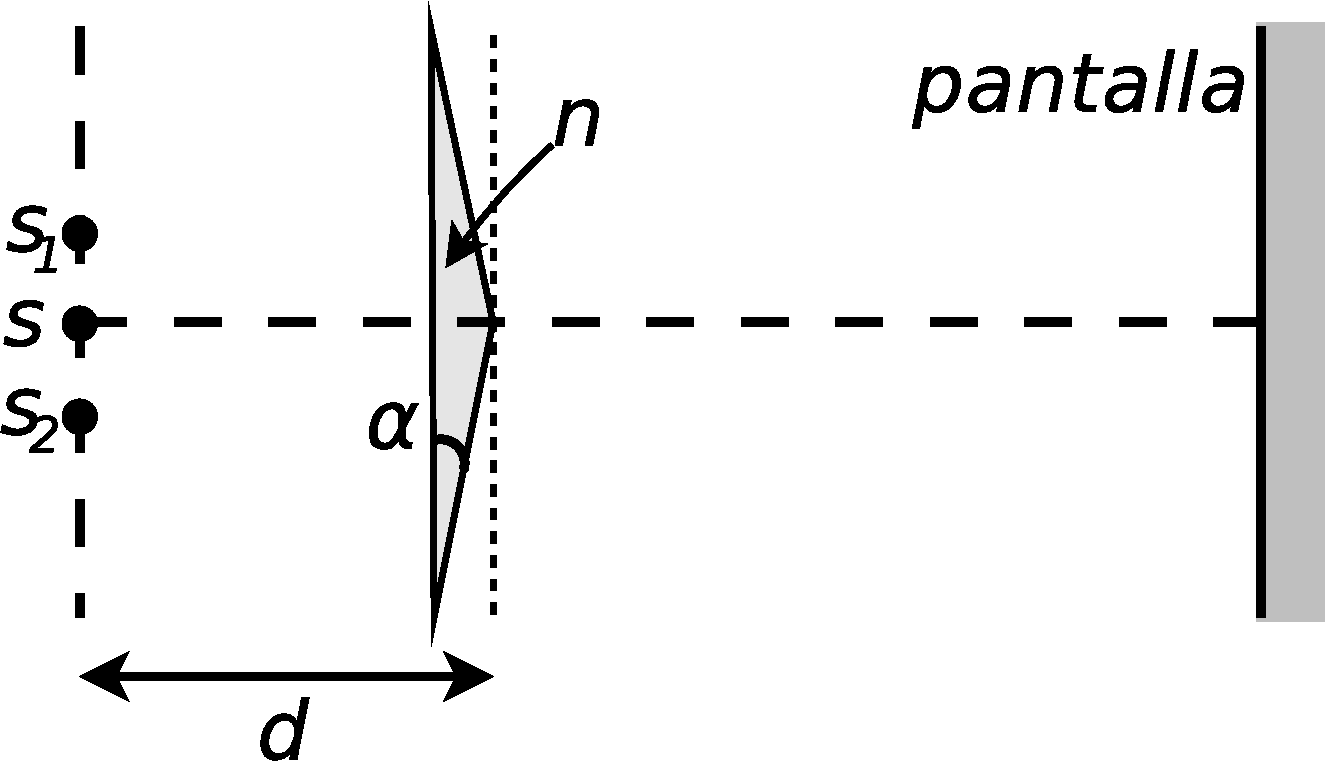
\includegraphics[width=\textwidth]{ej5-11}
\end{minipage}


\item En un experimento de interferencia con un biprisma de Fresnel, ¿qué
parámetros se pueden modificar para que la interfranja aumente?


\item
Se observan franjas de interferencia con un biprisma de Fresnel con
ángulo de $1.5{}^{\circ}$ e índice de refracción $1.5$. Para esto
se usa una fuente de luz de 4000 Å situada a 5 cm del vértice, y una
pantalla situada a 1 m del biprisma. Si, dejando todas las demás condiciones
iguales, se cambia el biprisma por uno de ángulo 3$^{\circ}$ e índice
$1.6$; ¿en cuánto varió la interfranja?


%\item 
%\begin{minipage}[t]{0.65\textwidth}
%Se tiene un dispositivo para producir interferencia consistente en
%una fuente puntual y monocromática $S$, que emite con longitud de
%onda $\lambda$, que se encuentra a una distancia $D_{1}$ de un biprisma
%compuesto por dos prismas delgados de distintos índices y ángulos:
%$n_{1}$, $\alpha_{1}$ ($y>0$) y $n_{2}$, $\alpha_{2}$ ($y<0$).
%\end{minipage}
%\begin{minipage}[c][1em][t]{0.3\textwidth}
%    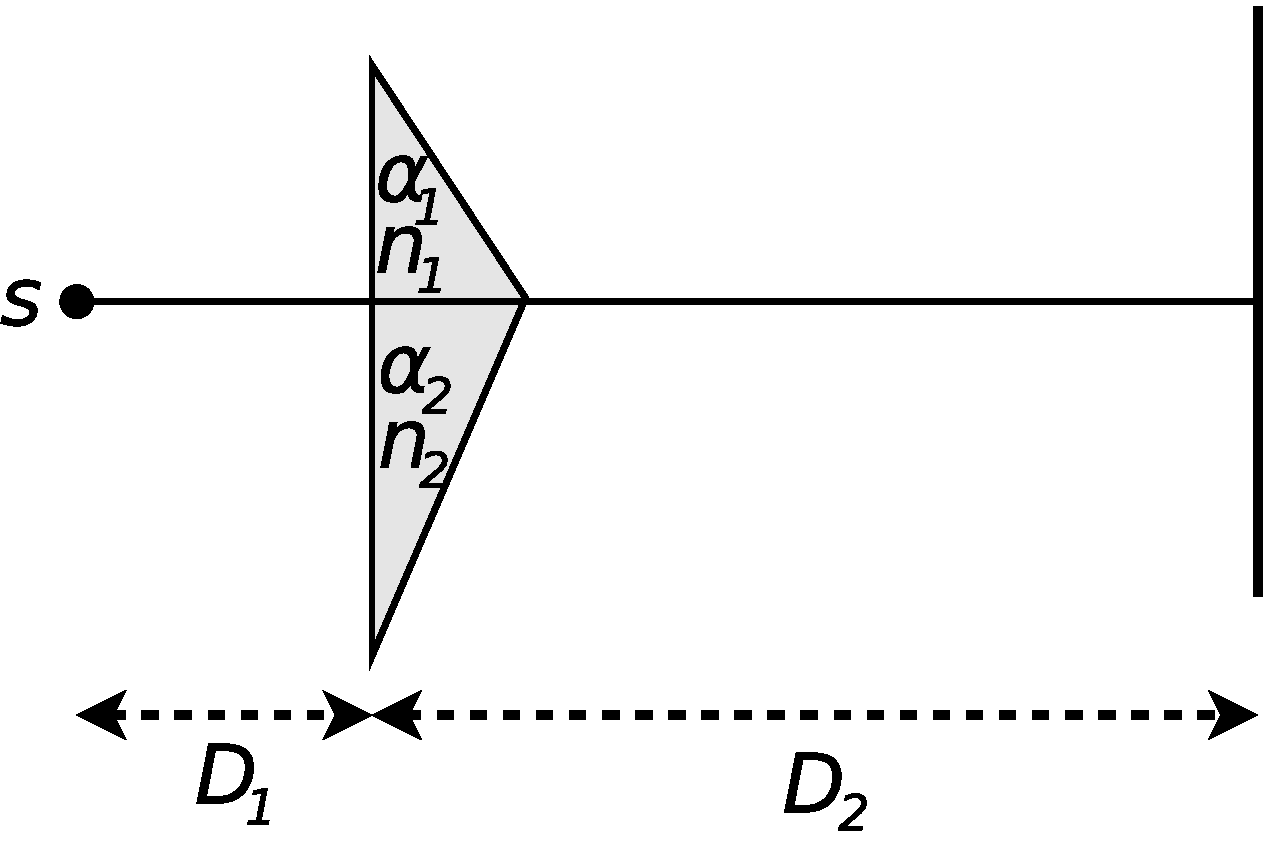
\includegraphics[width=\textwidth]{ej5-15}
%\end{minipage}



%\subsection*{Espejos}
%
%\item 
%Se usa como fuente luminosa para un par de espejos de Fresnel una ranura \(D\) iluminada con luz monocromática de \SI{400}{\nano\metre} colocada a \SI{20}{\centi\metre} de la intersección de los espejos sobre la bisectriz.
%Las franjas de interferencia observadas a \SI{1}{\metre} de distancia del vértice de los espejos tienen una interfranja de \SI{1}{\milli\metre}.
%Calcule el ángulo \(\alpha\) entre los planos de los espejos.
%Ayuda: note que \(S\) (fuente), \(S_1\) y \(S_2\) (imágenes de la fuente) equidistan de la intersección de los espejos.
%
%
%\item 
%En el experimento del espejo de Lloyd:
%\begin{enumerate}
%	\item diga cuáles son las dos fuentes coherentes que interfieren.
%	\item ¿Por qué motivo se puede concluir que la luz reflejada ha sufrido un desfasaje de 180º? 
%\end{enumerate}


\section*{Interferómetros por división de amplitud}

\subsection*{Láminas delgadas}
%
%\item
%\parbox[t]{\dimexpr\textwidth-\leftmargin}{%
%	\vspace{-2mm}
%	\begin{wrapfigure}[4]{l}{0.3\textwidth}
%		\centering
%		\vspace{-\baselineskip}
%		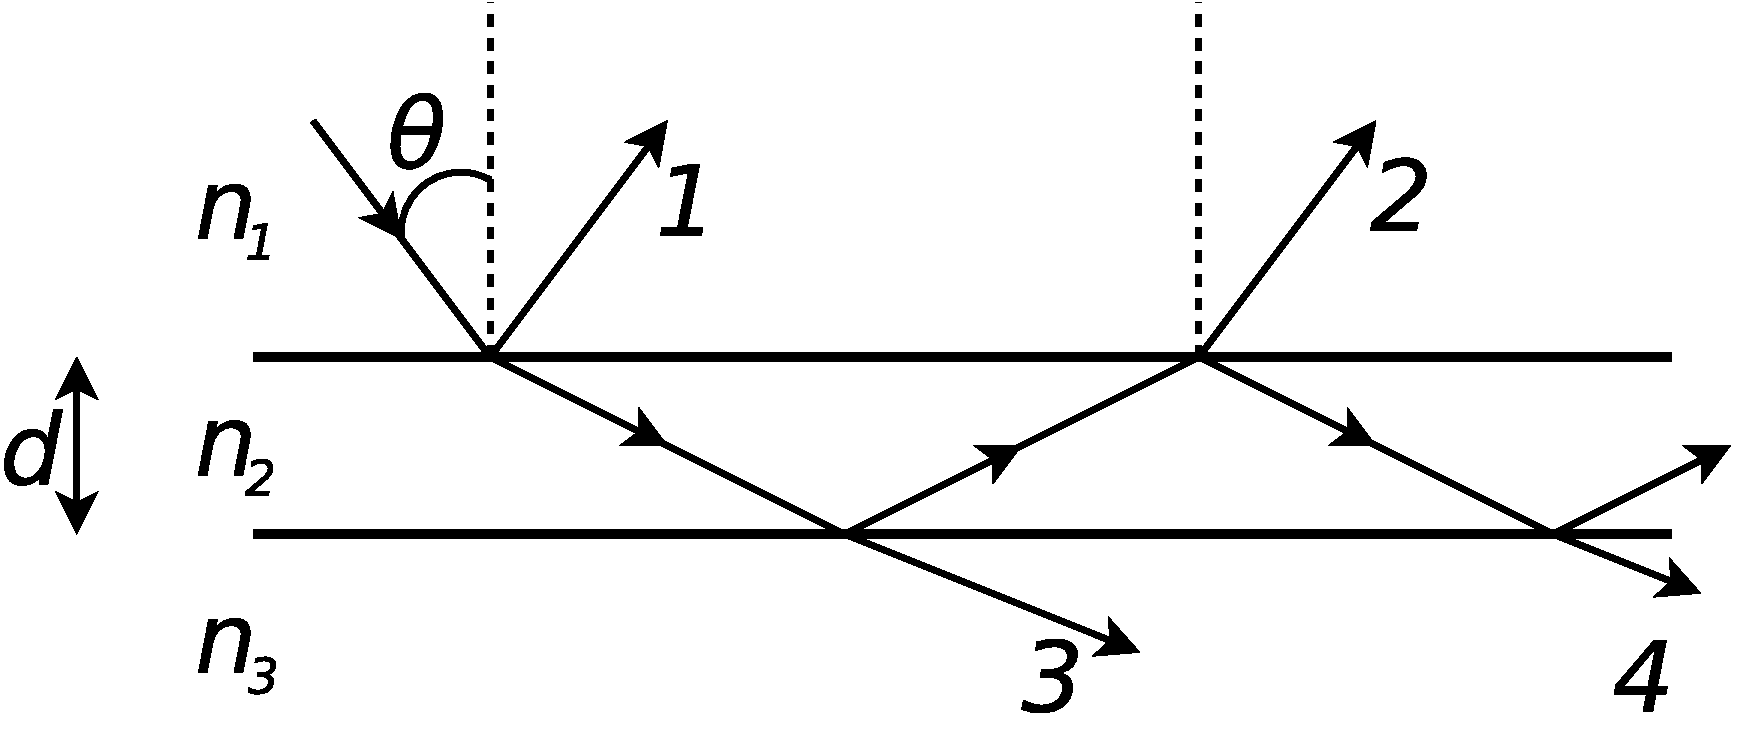
\includegraphics[width=\linewidth]{ej5-21}
%		% \caption{The beach}
%	\end{wrapfigure}
%	En la lámina de caras paralelas inmersa entre dos medios (\(n_1> n_2 > n_3\)) como se muestra en la figura:
%	\begin{enumerate}
%    	\item indique qué condición debe cumplirse para que los rayos \num{1} y \num{2} (correspondientes a la salida por reflexión) interfieran constructivamente.
%    	\item Cuando eso sucede, diga qué pasa con los rayos \num{3} y \num{4} (correspondientes a la salida por transmisión).
%    	\item ¿Qué sucede si se usan otras relaciones entre los índices?
%	\end{enumerate}
%}


\item
\begin{minipage}[t]{0.7\textwidth}
En la lámina de caras paralelas inmersa entre dos medios (\(n_1> n_2 > n_3\)) como se muestra en la figura:
\begin{enumerate}
	\item indique qué condición debe cumplirse para que los rayos \num{1} y \num{2} (correspondientes a la salida por reflexión) interfieran constructivamente.
	\item Cuando eso sucede, diga qué pasa con los rayos \num{3} y \num{4} (correspondientes a la salida por transmisión). ¿Qué sucede si se usan otras relaciones entre los índices?
\end{enumerate}
\end{minipage}
\begin{minipage}[c][1em][t]{0.25\textwidth}
	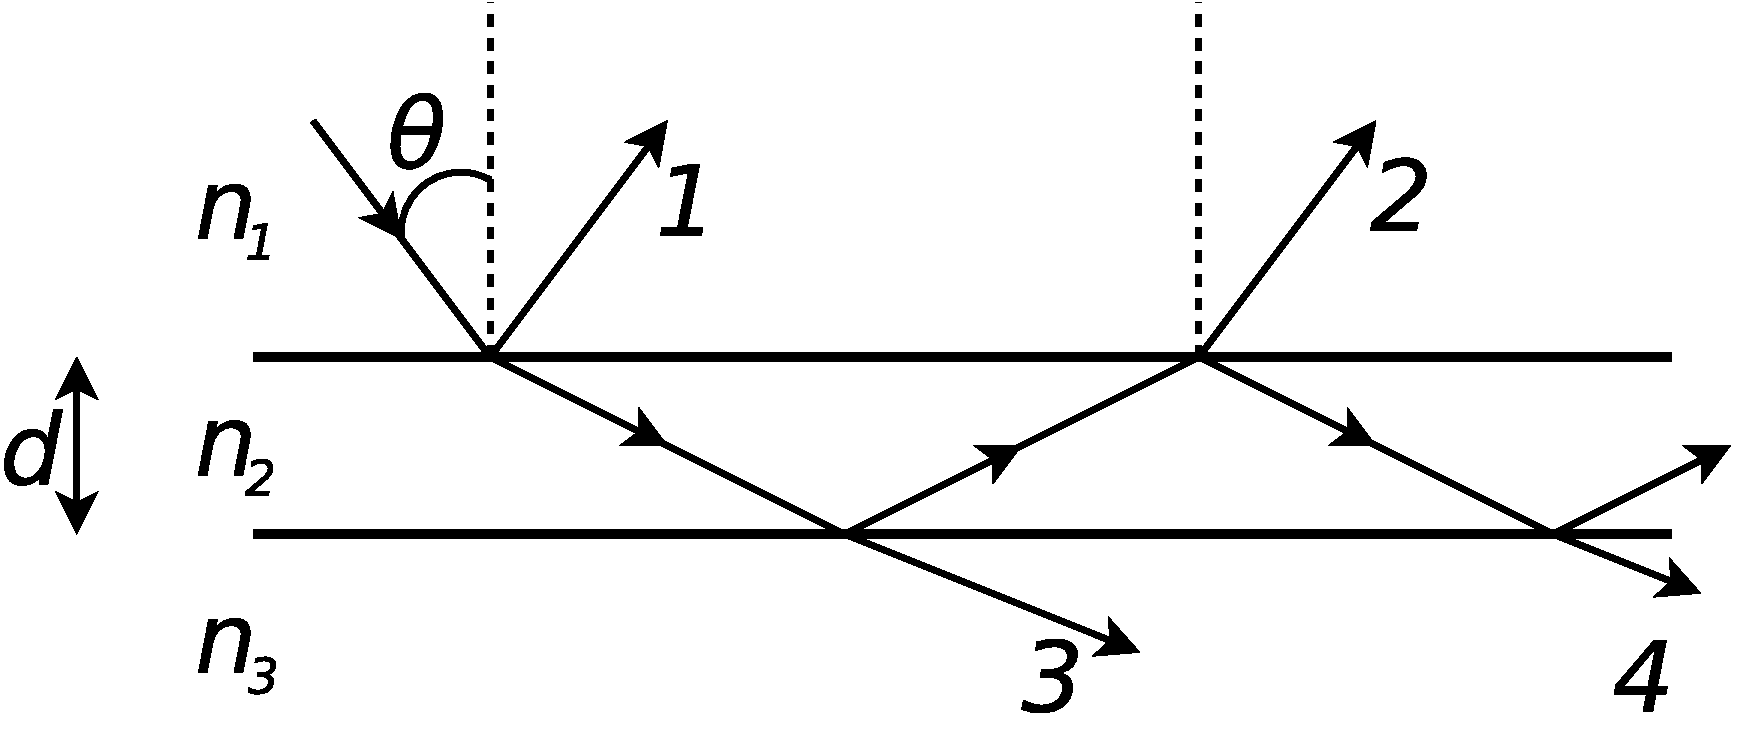
\includegraphics[width=\textwidth]{ej5-21}
\end{minipage}


%\item
%\begin{enumerate}
%	\item Determine el espesor de una lámina de jabón (\(n= 1.33\)) para una intensa reflexión de primer orden de la luz amarilla (\(\lambda= \SI{6000}{\angstrom}\) en el vacío).
%Suponga incidencia normal.
%	\item ¿Cuál es la longitud de onda de la luz en la lámina?
%\end{enumerate}


\item
Una lámina de vidrio de \SI{1.2}{\micro\metre} de espesor se ilumina con un haz de luz blanca normal a la lámina.
El índice de refracción del vidrio es \num{1.5}.
¿Qué longitudes de onda del espectro visible (de \SI{400}{\nano\metre} a \SI{700}{\nano\metre}) aparecerán intensificadas en el haz reflejado?


\subsection*{Cuñas}

\item
Sobre una delgada película en forma de cuña de plástico transparente, cuyo índice de refracción es \num{1.4}, incide normalmente luz monocromática.
El ángulo de la cuña es \SI{E-4}{\radian} y se observan franjas de interferencia con una separación de \SI{0.25}{\milli\metre} entre dos franjas brillantes continuas.
Calcule la longitud de onda (en el aire) de  la luz incidente.


%\item
%Una cuña de aire iluminada de tal forma que incide luz de longitud de onda (\(\lambda= \SI{500}{\nano\metre}\)) normalmente a la cara inferior, produce franjas paralelas cuya distancia entre mínimos es de \SI{1}{\milli\metre}.
%Describa la geometría de la cuña.


\item 
Un vidrio plano, con índice de refracción \(n_v=1.5\) está situado sobre un plástico plano de plástico con \(n_p=1.2\), y ambos se tocan en el punto A.
Desde arriba incide luz de \(\lambda= \SI{6000}{\angstrom}\).
\begin{enumerate}
	\item ¿Cuál de las dos figuras (b o c) es la que muestra el patrón de interferencia observado en la luz reflejada? (blanco \(\rightarrow\) máximo; negro \(\rightarrow\) mínimo)
	\item ¿Cuál es la separación entre el vidrio y el plástico en el punto B?
	\item Si la distancia entre A y B es de \SI{6}{\centi\metre}, ¿cuál es la densidad de franjas (expresado el resultado en franjas por metro)?
	\item Si la región entre el vidrio y el plástico se llena con agua (\(n_a=\frac{4}{3}\)), ¿cuántas franjas oscuras completas se ven ahora?
\end{enumerate}
\vspace{-.6cm}
\begin{center}
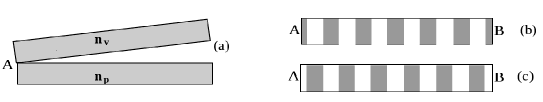
\includegraphics[width=0.75\textwidth]{itba25-10.png}
\end{center}



\subsection*{Anillos de Newton en lentes}

\item
Se observan anillos de Newton cuando una lente plano-convexa está colocada de modo que la cara convexa se apoya sobre una superficie plana de vidrio.
Se ilumina el sistema desde arriba con luz monocromática e incidencia casi normal.
El radio de la superficie convexa es de \SI{4}{\metre}.
\begin{enumerate}
	\item El radio del primer anillo brillante es de \SI{1}{\milli\metre} (se observa por reflexión).
Calcule la longitud de onda de la luz empleada.
	\item Se llena de agua el espacio comprendido entre la lente y la superficie plana de vidrio.
Calcule el radio del primer anillo brillante observado por reflexión. 
\end{enumerate}


\item En un dispositivo para observar anillos de Newton el espacio entre la lente y la lámina de vidrio está lleno de líquido.
Hallar el índice de refracción del mismo sabiendo que el radio del tercer anillo brillante es de \SI{3.65}{\milli\metre}.
La observación se hace por reflexión.
El radio de curvatura de la lente es de \SI{10}{\metre}.
La longitud de onda de la luz empleada es de \SI{589}{\nano\metre}.


\end{enumerate}
\end{document}
